\documentclass[msc,lith,english]{liuthesis}

%%%%%%%%%%%%%%%%%%%%%%%%%%%%%%%%%%%%%%%%%%%%%%%%%
% Imports
%%%%%%%%%%%%%%%%%%%%%%%%%%%%%%%%%%%%%%%%%%%%%%%%%
%\usepackage[english]{babel}
\usepackage[utf8]{inputenc}
\usepackage[backend=biber,sorting=none,hyperref]{biblatex}
\usepackage{mathtools}
\usepackage{dsfont}
\usepackage{tikz}
\usetikzlibrary{topaths,calc,tikzmark}
\usepackage{algorithm2e}
\usepackage{pgfgantt}

%%%%%%%%%%%%%%%%%%%%%%%%%%%%%%%%%%%%%%%%%%%%%%%%%
% Settings
%%%%%%%%%%%%%%%%%%%%%%%%%%%%%%%%%%%%%%%%%%%%%%%%%
\department{Institutionen för datavetenskap}
\departmentenglish{Department of Computer and Information Science}
\departmentshort{IDA}

\supervisor{Peter Jonson}
\examiner{???}
\titleenglish{A Faster Algorithm for Solving the No-Rainbow Problem}
% \subtitleenglish{100\% rainbow-free guarantee}
\titleswedish{En snabbare algoritm för No Rainbow problemet}
\thesissubject{Datavetenskap}

\publicationyear{2023}
\currentyearthesisnumber{001}
\dateofpublication{2023-01-20}

\addbibresource{thesis.bib}

\newcommand\tikznode[3][]%
   {\tikz[remember picture, baseline=(#2.base)]
      \node[minimum size=0pt,inner sep=0pt,#1](#2){#3};%
   }

\author{Edvard Thörnros}

\begin{document}

%%%%%%%%%%%%%%%%%%%%%%%%%%%%%%%%%%%%%%%%%%%%%%%%%
% Intro
%%%%%%%%%%%%%%%%%%%%%%%%%%%%%%%%%%%%%%%%%%%%%%%%%
\chapter{Introduction}
\label{chaIntro}
Decreasing the time commitment of something lets that thing be done a lot more often.
One part of this is finding faster algorithms for known hard problems.
Insight into hard problems, will also let us tackle even harder problems.
One such hard problem is the no rainbow problem.

The no rainbow problem \cite{sourceNoRainbow} asks if there is a surjective node coloring of an $r$-regular hyper graph.
Rephrased, the no rainbow problem asks if we can assign each node a color.
In a hyper graph with $r$ nodes per edge -- each edge connects $r$ different nodes.
All $r$ colors should be represented in the entire graph.
No edge should connect all $r$ colors.
A node coloring that satisfies these constraints is a solution to the no rainbow problem.

An edge that connects all $r$ colors is called a rainbow edge -- hence the name of the problem.
The no rainbow problem is a constraint satisfaction problem and is NP-complete.

\section{Motivation}
The no rainbow problem is related to the phylogenetic decisiveness problem \cite{sourceNoRainbow, sourcePhylogeneticDecisiveness}. The
phylogenetic decisiveness problem asks if a potential ancestral tree for a
species of animals could possibly be correct, given only parts of the
information about the ancestry of a species.
Understanding species will lead to a better understanding of the world.  

Solving problems is of general importance. Making current solutions faster is also helpful.
A solution to a problem can be reused in more complex problems. The more
efficient we can solve the first problem, the more efficient solutions built on
top of the first problem are. 

Some pieces of mathematics are seen as controversial at first until an application is found.
Negative numbers is an excellent example. Negative numbers were highly
controversial \cite{sourceNeg}. But today we commonly use imaginary numbers -- that is an extension of the negative numbers -- to
describe currents and rotations. Not all pieces of mathematics have obvious
applications when they are discovered. Graph theory and computer science are in
that sense very young fields.
The potential of future uses aside from phylogenetic decisiveness should not elude the reader.

% Honestly, this is grasping at straws.
The no rainbow problem is a studied NP-hard problem and could give some insight into the P versus NP problem.
The P versus NP problem is one of the millennium problems -- a solution would have enormous ramifications for our lives.
Though this algorithm might be simple, this improvement might be used as a
stepping stone in solving a central problem.

% TODO: Read https://ieeexplore.ieee.org/document/9616390
% TODO: https://www.researchgate.net/publication/350673538_Exact_Algorithms_for_No-Rainbow_Coloring_and_Phylogenetic_Decisiveness

\section{Research questions}
\begin{enumerate}
  \item Is there a faster* deterministic algorithm that solves the no rainbow problem than the one suggested by Ghazaleh Parvini and David Fernandez-Baca \cite{sourceNoRainbow}?
  \item Is there a faster* randomized algorithm that solves the no rainbow problem than the one suggested by Ghazaleh Parvini and David Fernandez-Baca \cite{sourceNoRainbow}?
  % \item How can a solution to the no rainbow problem be found, understood, modeled and presented?
  % \item What insights into algorithms are found by studying the no rainbow problem?
  \item How fast* is the fastest* possible algorithm for solving the no rainbow problem? 
\end{enumerate}
*Speed is defined by asymptotic computational complexity.

\section{Aim}
The aim of this study is to find an asymptotically faster algorithm that solves
the no rainbow problem. The algorithm should then be presented and evaluated.
This new algorithm should make it easier to solve the phylogenetic decisiveness
problem and any other potential problem that can be mapped to it.

\section{Delimitations}
This study will focus on the theoretical no rainbow problem.
Implementing the algorithms is not part of this study.
This article is theoretical.

%%%%%%%%%%%%%%%%%%%%%%%%%%%%%%%%%%%%%%%%%%%%%%%%%
% Background
%%%%%%%%%%%%%%%%%%%%%%%%%%%%%%%%%%%%%%%%%%%%%%%%%
\chapter{Background}
\label{chaBackground}
The no rainbow problem is quite complex and can be understood in a lot of different ways.
To understand the problem as broadly as possible a few different areas of discrete mathematics are needed.

% \section{Equivalence classes and equivalence relations}
% Equivalence classes are used to group things that are equal in some sense.
% This requires we have a set of objects and an binary operator we can use to check if they are equal.
% In this general case we use $\sim$ as the operator.
% 
% $$
%   a \sim b \implies \textit{$a$ is related to $b$ under the equivalence relation ($\sim$)}
% $$
% 
% A common way of defining equivalence relations is to map the objects to their image and then use equality.
% More generally we can define it using:
% $$
%   a \sim b \iff f(a) = f(b)
% $$
% Where $f(a)$ is the image of $a$.
% 
% For example:
% $$
%   a \sim b \iff (a \bmod 3) = (b \bmod 3) : \quad a, b \in \mathds{Z}
% $$
% 
% Here we send each object to their image -- that is their remained after division by 3 -- and then compare them.
% Here we get 3 equivalence classes $\{[0], [1], [2]\}$. All integers are mapped into exactly one of these 3 equivalence class.
% 
% The representative of a class is the element that has itself as image. In other words, $f(a) = a \iff a$ is a representative.
% \cite[Section 7.3]{sourceArmen} \cite[Section 1.2]{sourceAATA}

\section{Graphs}
Graphs consist of a set of edges and a set of nodes
% \cite[Chapter 1]{sourceDiestel}
% \cite[Chapter 1]{sourceGWA}
\cite[Section 9.1]{sourceArmen}.

Nodes are usually presented as circles with edges connecting the circles as lines, as presented in Figure \ref{figGraphExample}.
Usually an edge is some kind of relationship. 
A graph is a very powerful and general tool for modeling many problems.

\begin{center}
\begin{figure}[h]
\centering
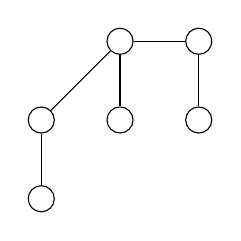
\begin{tikzpicture}[main/.style = {draw, circle}]
    \node[main] (A) {};
    \node[main] (B) [left of=A] {};
    \node[main] (C) [below of=A] {};
    \node[main] (D) [left of=C] {};
    \node[main] (E) [left of=D] {};
    \node[main] (F) [below of=E] {};

    \draw (A) -- (B);
    \draw (A) -- (C);
    \draw (B) -- (D);
    \draw (B) -- (E);
    \draw (F) -- (E);
\end{tikzpicture}
  \caption{An example of a graph.}
  \label{figGraphExample}
\end{figure}
\end{center}

% Does this add anything?

\section{Hyper Graphs}
A hyper graph is similar to a normal graph.
All edges in a hyper graph connect multiple nodes, usually more than 2.
A hyper edge that is 2-regular is a ``normal`` graph.
The ``normal`` graph can be seen as a special case of the hyper graph.
Another way of phrasing it is that an edge is a set of nodes instead of a pair.

A hyper graph is the kind of graph the no rainbow problem.

\begin{center}
\begin{figure}[h]
\centering
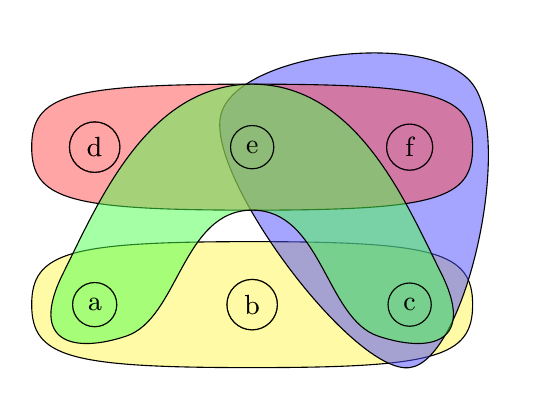
\begin{tikzpicture}[main/.style = {draw, circle}]
    \node[main] (a) at (0,2) {a};
    \node[main] (b) at (2,2) {b};
    \node[main] (c) at (4,2) {c};
    \node[main] (d) at (0,4) {d};
    \node[main] (e) at (2,4) {e};
    \node[main] (f) at (4,4) {f};

    \begin{scope}[fill opacity=0.5]
    \filldraw[fill=yellow!70] 
        plot [smooth cycle, tension=1.5]
        coordinates {
          ($(a)+(-0.8,0)$) 
          ($(b)+(0,0.8)$) 
          ($(c)+(0.8,0)$)
          ($(b)+(0,-0.8)$) 
        };

    \filldraw[fill=blue!70] 
        plot [smooth cycle, tension=0.8]
        coordinates {
          ($(c)+(0,-0.8)$) 
          ($(f)+(0.8,0.8)$) 
          ($(e)+(-0.4,0.4)$)
        };

    \filldraw[fill=red!70] 
        plot [smooth cycle, tension=1.5]
        coordinates {
          ($(d)+(-0.8,0)$) 
          ($(e)+(0,0.8)$) 
          ($(f)+(0.8,0)$)
          ($(e)+(0,-0.8)$) 
        };

    \filldraw[fill=green!70] 
        plot [smooth cycle, tension=1.0]
        coordinates {
          ($(c)+(-0.4,-0.4)$) 
          ($(c)+(0.4,0.4)$) 
          ($(e)+(0,0.8)$)
          ($(a)+(-0.4,0.4)$) 
          ($(a)+(0.4,-0.4)$) 
          ($(e)+(0,-0.8)$)
        };

    \end{scope};

    \node[main] (a) at (0,2) {a};
    \node[main] (b) at (2,2) {b};
    \node[main] (c) at (4,2) {c};
    \node[main] (d) at (0,4) {d};
    \node[main] (e) at (2,4) {e};
    \node[main] (f) at (4,4) {f};
\end{tikzpicture}
  \caption{An example of a hyper graph.}
  \label{figHyperGraphExample}
\end{figure}
\end{center}

% Show the other way of rendering them

The hyper graph shown in Figure \ref{figHyperGraphExample} is $3$-regular.
A hyper graph is $r$-regular if and only if all edges connect $r$-different nodes.
\cite{sourceHyper}

\section{Node coloring as related by the no rainbow problem}
A node coloring is a mapping from nodes to colors.
There are usually constraints on what colors can be part of an edge.
The color of a node is denoted as $c(a)$, where $a$ is the node and $c$ is the coloring.
Since a coloring is a mapping it can be thought of as a function that takes you from a node to the color of the node.
A color is usually a letter or a number.

The constraints added in the no rainbow problem are
\begin{enumerate}
  \item No edge can have all r-colors -- no rainbow edges
  \item All colors have to be represented in the graph -- the coloring is surjective
\end{enumerate}

An example of a valid coloring in the no rainbow problem for the graph presented above is $c(d)=0, c(b)=1, c(*)=2$, where $*$ denotes all other nodes.
There are a lot more valid colorings, though this coloring is particularly simple.
The validity of a coloring is dictated by the edges added in the graph.
A hyper-graph with the maximum number of edges (called a complete graph) has no valid no-rainbow coloring.
A hyper-graph without any edges is trivial to find a no-rainbow coloring for.
The cases in between are the main topic of this thesis.

\cite{sourceHyper}
% Is a complete r-regular subgraph enough to disprove there is a no-rainbow coloring? Yes.

\section{Asymptotic Computational Complexity}
Sometimes called asymptotic time complexity is a theoretical basis for evaluating algorithms.
The asymptotic computational complexity of an algorithm shows how the run time
of the implemented algorithm scales given infinitely large inputs.


There are multiple kinds of asymptotic computational complexity \cite[Chapter 3]{sourceAlgoBook}. The most used
one -- and the one presented in this paper -- is the ``big-O`` notation. ``Big-O``
gives the highest upper bound of this theoretical runtime -- or the worst-case
computational complexity. Examples usually make things clearer, so let us look at an algorithm.
One intuition for the computational complexity is to ``count the number of steps``.

\begin{algorithm}
\caption{A slow exponentiation algorithm.}\label{algDivSlow}
\KwData{$a,b \in \mathds{Z}, \quad b \le 0$}
\KwResult{$a^b$}
\DontPrintSemicolon
\SetKwFunction{FExp}{Exp}
\SetKwProg{Fn}{Function}{:}{end}

\Fn{\FExp{$a$, $b$}}{
  $x \gets 1$ (Runs 1 time.)\;
  \While(\lparen Runs $b$ times, with $K$ steps.\rparen){$b \le 0$}{
    $x \gets x * a$\; 
    $b \gets b - 1$\;
  }
  \KwRet $x$ (Runs 1 time.)\;
}
\end{algorithm}

We assume multiplication can be done in constant time -- it always takes at most $K$ units of time to do a multiplication.
The Algorithm \ref{algDivSlow} will perform $ 2 + Kb $ steps, where $K$ is some
constant. We can rewrite this using ``Big-O`` notation as $O(1 + Kb)$. The expression can be
simplified to remove constants that become insignificant if the
input is sufficiently large. Then we get $O(2 + Kb) = O(b)$, since both $1$ and $K$ are constants. 
Normally the asymptotic time complexity is defined based on the size of the input not the magnitude of the value.
The size of the input is measured in number of bits called $n$. When we add a bit to $b$ we multiply the steps by 2,
thus $O(b) = O(2^n)$.

There are other ways to reason to this conclusion.
One other way is to realize we have to visit all numbers between $0$ and $b$.
In binary this means visiting all possible combinations of 0s and 1s that are needed to describe $b$.
We have 2 choices for $n$ bits. All combinations have to be visited. So we visit $O(2^n)$ numbers in the worst case. 

A common error is to claim Algorithm \ref{algDivSlow} runs in $O(n)$ -- linear time. This is incorrect.

Aside from $O$ there is also $O^*$. $O^*(x^n)$ allows us to discard polynomial factors as well. For example $O^*(x^n)$ would allow the algorithm to run in $O(P(x)x^n)$ where $P(x)$ is some polynomial.

\section{Constraint Satisfaction Problems}
Constraint satisfaction problems -- often called CSPs -- is a kind of mathematical problem where a finite set of constraints should be fulfilled. Let us consider some examples of these problems.

One very relevant kind of constraint satisfaction problem is node coloring of hyper graphs.
Constraints are put on what colors can be put where. In the no rainbow problem all colors should never be part of an edge, but all colors should be present in the graph. What makes this problem tricky is that changes locally (to the nodes in an edge) can affect other parts of the graph -- since a node can be part of multiple edges.

Another well known constraint satisfaction problem is SAT -- that is further discussed in Section \ref{secSAT}.

\section{SAT, k-SAT and 3SAT}\label{secSAT}
SAT is a very central problem in theoretical computer science. 3SAT is the
hinge pin on that P versus NP rests -- an efficient algorithm for solving 3SAT
solves P versus NP.

SAT, k-SAT and 3SAT ask if logical formulas are satisfiable (there is an assignment in that the expression is true).
The difference between the 3 problems is the input. SAT takes any formula in
CNF-format (conjunctive normal form) -- all clauses are separated by conjunctions and
in clauses only negation, variables and disjunction are allowed.

$$
  (\tikzmark{v1}a\tikzmark{v2} \vee b \vee c) \tikzmark{w1}\wedge\tikzmark{w2} (\overline{c} \vee d \tikzmark{o1}\vee\tikzmark{o2} e) \wedge \tikzmark{c1}(a \vee \overline{c} \vee e)\tikzmark{c2}
$$
\begin{figure}[h]

\begin{tikzpicture}[overlay, remember picture, main/.style = {}]
  
  \node[main, color=blue] (var) at (4,0.3) {variable};
  \node[main, color=green] (conj) at (6,0.3) {conjunction};
  \node[main, color=red] (clause) at (10,0.3) {clause};
  \node[main, color=cyan] (dis) at (8.3,0.3) {disjunction};

  \draw[-, line width=3mm, opacity=0.5, color=blue] ([yshift=1mm]pic cs:v1) -- ([yshift=1mm]pic cs:v2);
  \draw[-, line width=3mm, opacity=0.5, color=green] ([yshift=1mm]pic cs:w1) -- ([yshift=1mm]pic cs:w2);
  \draw[-, line width=3mm, opacity=0.5, color=red] ([yshift=1mm]pic cs:c1) -- ([yshift=1mm]pic cs:c2);
  \draw[-, line width=3mm, opacity=0.5, color=cyan] ([yshift=1mm]pic cs:o1) -- ([yshift=1mm]pic cs:o2);

  \draw[color=blue] (var) -- (pic cs:v1);
  \draw[color=green] (conj) -- (pic cs:w1);
  \draw[color=red] (clause) -- (pic cs:c1);
  \draw[color=cyan]  (dis) -- (pic cs:o1);

\end{tikzpicture}
  \caption{A labeling of a logical expression. An example of input to 3SAT.}
  \label{figExSAT}
\end{figure}


An example labeling of the  parts of a logical expression is seen in Figure
\ref{figExSAT}. 3SAT requires all clauses to have exactly 3 variables. k-SAT requires all clauses to have exactly k variables. SAT puts not constraints on the causes. But the formula has to be in conjunctive normal form (CNF).




\chapter{Related Work}
Exhaustive studies of the no rainbow problem have not been done. There are however a plethora of related problems.
These related problems are more broadly studied. This section gives insight
into these related works. In particular there is a review of the currently
fastest algorithms.

\section{Exact Algorithms for No-Rainbow Coloring and Phylogenetic Decisiveness}
``Exact Algorithms for No-Rainbow Coloring and Phylogenetic Decisiveness`` \cite{sourceNoRainbow}
are currently the fastest algorithms.
Two algorithms are presented. One deterministic and one non-deterministic. Both
algorithms use the idea of searching similar potential solutions for a fixed
depth, and then trying again. The non-deterministic algorithm samples the
solution space randomly, while the deterministic algorithm samples a specific
structure. The different search patterns are visualized in Figure \ref{figNoRainbowSearchPattern}. 

The paper by \citeauthor{sourceNoRainbow} \cite{sourceNoRainbow} is a great starting point for finding a faster algorithm.
Adapting the algorithm to lean more into hyper graphs might give valuable insights into the problem to speed it up.
In the paper the mathematics and proofs are described. There is no method section in this paper.

\begin{center}
\begin{figure}[h]
\centering
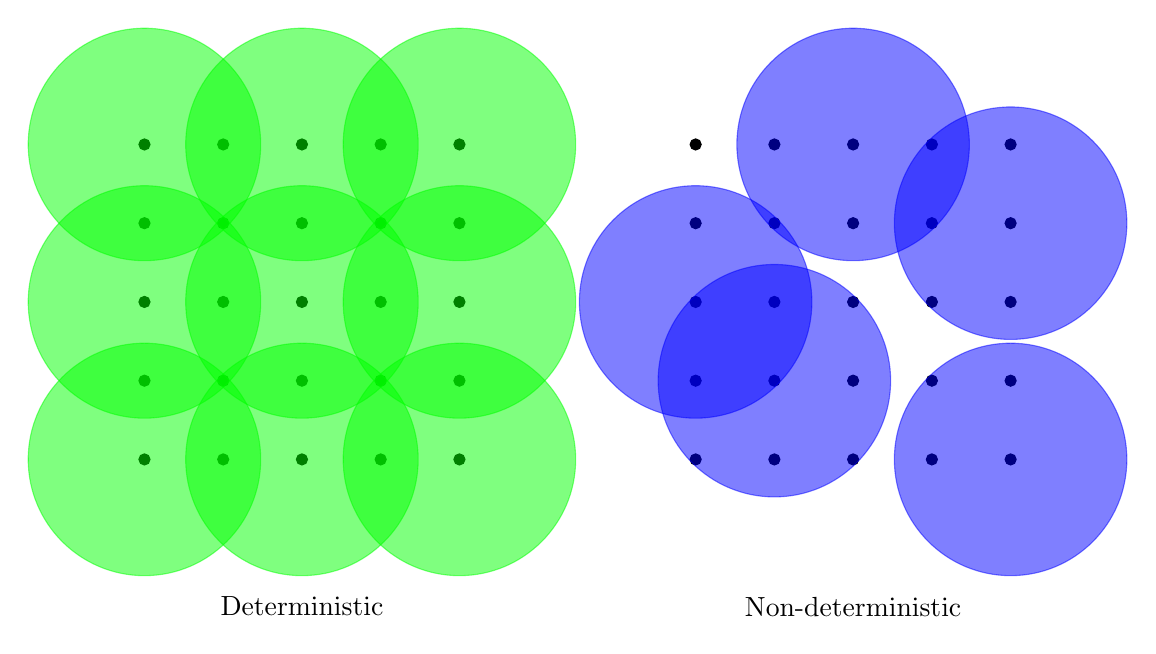
\begin{tikzpicture}
  \newcommand\circleRadius{42pt}

  \foreach \x in {0,...,4}{
    \foreach \y in {0,...,4}{
      \filldraw[black] (\x,\y) circle (2pt);
    }
  }

  \foreach \x in {0,2,4}{
    \foreach \y in {0,2,4}{
      \filldraw[green, opacity=0.5] (\x,\y) circle (\circleRadius);
    }
  }
  \draw (2,-1.5) node[label=below:Deterministic]{};

  % SHIFTED +(4+3,0)
  \foreach \x in {7,...,11}{
    \foreach \y in {0,...,4}{
      \filldraw[black] (\x,\y) circle (2pt);
    }
  }

  \filldraw[blue, opacity=0.5] (8,1) circle (\circleRadius);
  \filldraw[blue, opacity=0.5] (7,2) circle (\circleRadius);
  \filldraw[blue, opacity=0.5] (11,0) circle (\circleRadius);
  \filldraw[blue, opacity=0.5] (9,4) circle (\circleRadius);
  \filldraw[blue, opacity=0.5] (11,3) circle (\circleRadius);
  \draw (9,-1.5) node[label=below:Non-deterministic]{};


\end{tikzpicture}
  \caption{A visualization of how the deterministic and non-deterministic algorithms tries different colorings. Each black dot is a potential solution. The colored circles show the searched adjacent solutions.}
  \label{figNoRainbowSearchPattern}
\end{figure}
\end{center}

\section{A Probabilistic Algorithm for k-SAT and Constraint Satisfaction Problems}
\citeauthor{sourceProbAlgo} \cite{sourceProbAlgo} propose a very simple algorithm for solving k-SAT.
The algorithm is then generalized to all constraint satisfaction problems. The
algorithm is faster than most of the known algorithms of the time and is
similar to the algorithm proposed by \citeauthor{sourceNoRainbow} \cite{sourceNoRainbow}.

In the paper there is no method section. The algorithm is simply presented and proven very well. 

The k-SAT algorithm randomly flips assignments for variables in constraints that are not satisfied.
How k-SAT searches is visualized in Figure \ref{figKSATSearch}.

\begin{center}
\begin{figure}[h]
\centering
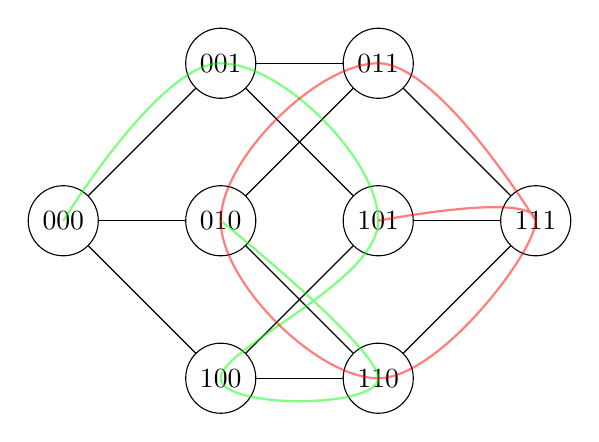
\begin{tikzpicture}[node/.style = {draw, circle}, scale=2]
  \node[node] (a000) at (0,0) {000};

  \node[node] (a001) at (1,1) {001};
  \node[node] (a010) at (1,0) {010};
  \node[node] (a100) at (1,-1) {100};

  \node[node] (a011) at (2,1) {011};
  \node[node] (a101) at (2,0) {101};
  \node[node] (a110) at (2,-1) {110};
  
  \node[node] (a111) at (3,0) {111};

  \draw (a000) -- (a001);
  \draw (a000) -- (a010);
  \draw (a000) -- (a100);

  \draw (a011) -- (a001);
  \draw (a101) -- (a001);

  \draw (a110) -- (a010);
  \draw (a011) -- (a010);

  \draw (a110) -- (a100);
  \draw (a101) -- (a100);

  \draw (a011) -- (a111);
  \draw (a101) -- (a111);
  \draw (a110) -- (a111);

  \draw[opacity=0.5, thick, smooth, tension=0.7, green] plot[line width=5mm] coordinates { (a000) (a001) (a101) (a100) (a110) (a010) };
  \draw[opacity=0.5, thick, smooth, tension=0.7, red  ] plot[line width=5mm] coordinates { (a101) (a111) (a110) (a010) (a011) (a111) };

\end{tikzpicture}
\caption{A visualization of how the k-SAT algorithm would search for solutions when there are 3 variables. Each node is a potential variable assignment. The lines show how the assignments are searched. The red line is one search and the green line is another search.}
\label{figKSATSearch}
\end{figure}
\end{center}

\section{Survey Propagation: an Algorithm for Satisfiability}
\citeauthor{sourceSurveyProp} \cite{sourceSurveyProp} suggest an algorithm that generalizes knowledge about parts of solutions of a SAT-problem. 
When the authors looked at the solution space, they noticed solvers often got stuck in local optimums.
These local optimums forced some variable assignments and created a form of cluster.
By surveying these clusters and generalizing the assignments better guesses can be made.
After iterating a good solution can be found by little effort.
Survey Propagation has no guarantees on convergence, but performs really well in practice.

There is no method chapter, only arguments and thoughts about the algorithm.

\section{On the Solution-Space Geometry of Random Constraint Satisfaction Problems}
The run time performance of an implementation of survey propagation is mentioned to perform incredibly well.
They even have such strong claims as:
\blockquote{No other algorithm practically solves formulas of such density with $n=10^4$.}
\cite{sourceSolutionSpace}

The run time speed of survey propagation is then discussed throughout the paper.
Informal claims for the run time performance are made with a basis of mathematical reasoning.
Further, reasoning of how solutions to constraint satisfaction problems and SAT cluster are made.
Concepts like ``frozen variables`` are introduced - variables which only have one
possible value given the current configuration, a sort of deadlock.

There is no method section in this paper.

\chapter{Project Plan}
An outline of the project plan is presented and the method to be used is discussed.

\section{Method}
The methodology of mathematics is not a well published subject \cite{sourceMethodMath}.
There is currently an internal debate in algorithms research \cite{sourceUllman}, debating the value of measuring implementations of algorithms.
Some benefits of theoretical analysis is the rigor of mathematics and the solid foundations it offers, but these are also theoretical constructs which might not map to reality \cite{sourceAlgorithmEngineeering}.
There are also heuristic solutions to problems which in practice perform better than algorithms with guarantees \cite{sourceSolutionSpace,sourceSurveyProp}.

The method most used in the papers is rigorous mathematical proofs. There might be value in coupling mathematics with run time evaluations of program implementations.
Small test implementations of the algorithms might also easily filter out obviously bad ideas given a sufficient amount of test cases.
Further, the methods in previous papers all center on mathematical arguments and problem-solving.

A good method would be a creative process of problem-solving and formulating the findings as mathematical proofs.
Since this method is what all other papers in this area are using.
There might be modifications that can be made to more suite a thesis in engineering,
but I am hesitant to try a novel methodology.

\section{GANTT-chart}
A GANTT-chart of the work is presented in Figure \ref{figGanttChart}.

\begin{center}
\begin{figure}[h]
\begin{ganttchart}[
    vgrid,
    bar left shift=0.15,
    bar right shift=-0.15,
    bar/.append style={rounded corners=3pt},
    bar inline label node/.style={%
      anchor=south, font=\ganttvalueof{bar label font}%
    },%
    inline,
    milestone inline label node/.style={%
      anchor=north, font=\ganttvalueof{milestone label font}%
    },%
    expand chart=\textwidth
]{1}{20}
\gantttitle{Project Plan}{20} \\
\gantttitlelist{1,...,20}{1} \\

\ganttgroup{Problem}{1}{13} \\
\ganttbar{Discover solutions}{1}{9}
\ganttlinkedbar{Present solution}{10}{13} \\
\ganttmilestone{Show to examiner}{4}
\ganttmilestone[milestone inline label node/.style={anchor=south}]{Solution OK by examiner}{9} \\
\\
\ganttgroup{Report}{1}{19} \\
\ganttbar{Related works}{2}{8} \\
\ganttbar{Discussion}{11}{13} \\
\ganttbar{Conclusion}{14}{14} \\
\ganttbar{Introduction}{15}{15} \\

\ganttbar{Polish report}{16}{17} \\
\ganttlinkedbar{Presentation}{18}{20} \\

\ganttmilestone{Find opponent}{16} \\
\ganttmilestone{1st hand in}{17} \\

\ganttmilestone[milestone inline label node/.style={anchor=north east}]{Hold presentation and final hand in}{20} \\

\ganttlink{elem1}{elem7}
\ganttlink{elem7}{elem8}
\ganttlink{elem6}{elem7}
\ganttlink{elem8}{elem9}
\ganttlink{elem9}{elem10}
\end{ganttchart}
  \caption{The project plan for the final thesis.}
  \label{figGanttChart}
\end{figure}
\end{center}

\subsection{Polish report}
In the report group, each task corresponds to a chapter except ``Polish report``.
The ``Polish report`` chapter is for fixing everything else that needs fixing.
The vague heading ``Polish report`` will also serve as slack for the project.

\subsection{Related works}
Reading of background and related material. This activity results in a finished background/related works section.
The background and related works should preferably be too long here to be trimmed shorter later.

\subsection{Discussion}
The discussion is written here.

\subsection{Conclusion}
The conclusion is written here.

\subsection{Introduction}
The Introduction is written here.

\subsection{Discover solutions}
The heading ``Discover solutions`` also needs some clarification. Constructing
an algorithm is a creative process. For a creative process it is instrumental
to move between working and thinking. Related works section is scheduled for
parts of the duration of discovering solutions. Since knowing more about the
area will feed back into new ideas for other algorithmic solutions. 
Figure \ref{figCreativeProcess} contains a visualization of the flow.

\begin{center}
\begin{figure}[h]
\centering
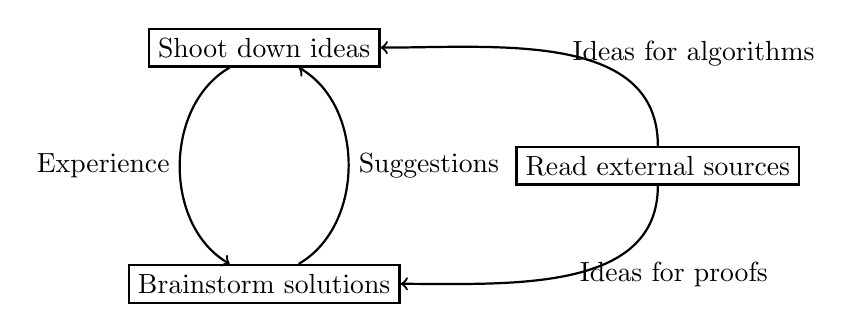
\begin{tikzpicture}[thick, node/.style = {draw}]
  \node[node] (a) at (0,0) {Brainstorm solutions};
  \node[node] (b) at (0,3) {Shoot down ideas};
  \node[node] (c) at (5,1.5) {Read external sources};

  \draw[->] (a) to[out=30,in=-30] node[right]{Suggestions} (b);
  \draw[->] (b) to[out=-150,in=150] node[left]{Experience} (a);
  \draw[->] (c) to[out=-90,in=0] node[right]{Ideas for proofs} (a);
  \draw[->] (c) to[out=90,in=0] node[right]{Ideas for algorithms} (b);
\end{tikzpicture}
\caption{The creative process of constructing algorithms according to the author.}
\label{figCreativeProcess}
\end{figure}
\end{center}

\subsection{Present solution}
Extra work is put into presenting the solution as well as possible.
This means polishing the proof to make the proofs as clear and well written as possible.
Here the bulk of the report is written. The proofs and the explanations are put into place.

\subsection{Milestones ``Show to examiner`` and ``Solution OK by examiner``}
These milestones will give me deadline.
These deadlines stop the creative process of discovering algorithms from losing focus.
I will know if these milestones are reached if my examiner thinks the work is looking acceptable.
These correspond to halftime reviews.

\subsection{Milestone ``Find opponent``}
Will find someone to oppose me, and preferably someone to oppose. 

\subsection{Milestone ``1st hand in``}
A first version of the thesis is handed in, in a state that I would be happy to
publish. But expecting further revisions.

\subsection{Milestone ``Hold presentation and final hand in``}
The final presentation is held. I get feedback from my examiner and my
opponent. This feedback is the quickly revised then the thesis can be sent for
publishing.

\subsection{Risks}

\begin{enumerate}
  \item (likelihood: medium, severity: high)
    The largest risk for failure in the plan. If no sufficiently good algorithm
    is found the project will have to be restructured. Either a different problem
    will have to be chosen (preferably in a related area), or the thesis will have
    to pivot to motivate why there is not a faster algorithm.

  \item (likelihood: low, severity: medium)
    The examiner might not know enough about the subject area to give valid
    guidance. This might prolong the project and force me to redo work. I will
    have to be critical of the feedback from my examiner and make sure I have a
    solid understanding.

  \item (likelihood: medium, severity: low)
    There might not be enough background surrounding the No Rainbow problem.
    This will force me to branch out more in my research but should still allow
    me to formulate a good thesis. The project might take more time if there
    are few sources. To mitigate this I should read a wide variety of articles.
\end{enumerate}

\printbibliography

\appendix
\chapter{Changes after feedback seminar (2022-11-25)}
Removed 2 research questions. Added motivation. Added aim. Added delimitations. Fixed typos of multi graph and hyper graph. Corrected typo in title. Moved background to its own chapter. Took feedback from Don and replaced ``which`` with ``that``.

\chapter{Changes after seminar 3 (2022-12-01)}
Reworded some sentences and fixed some typos. Changed source to adhere to the IEEE standard.

\chapter{Changes after seminar 5 (2022-12-16)}

\begin{itemize}
  \item Algorithm is spelled correctly in the title
  \item Slim down on graph references
  \item Method citations made clearer
  \item Method is clearified and expanded
  \item Introduction is streamlined
  \item CSP missing reference is fixed. 
  \item Related works is expanded to make relation to this thesis clearer
  \item Add deadlines from IDA
  \item Minor style language fixes
  \item Section on equivalence classes was removed since it is now unreferenced
  \item Added references to unreferenced figure
  \item Minor style touch ups
\end{itemize}

\end{document}
